\chapter{Controlled Production-to-Primary-CMB Einstein--Boltzmann Dynamics}
\label{ch:production-primary-cmb}

\section{Scope and objective}

The scale-covariant refinement dark sector now supplies a mass spectrum, a production distribution, a cold late-time limit, a collisionless perturbation hierarchy, and controlled late-time matter and lensing observables.  The remaining major linear-cosmology gap was the interval between production and last scattering.  In particular, the preceding late-time calculation did not jointly evolve photon collisions, polarization, baryons, massless neutrinos, metric driving, recombination, and the massive refinement hierarchy.

This chapter constructs that coupled system.  It evolves one unchanged dark-sector parameter set from
\begin{equation}
 a_{\star}=10^{-6}
 \label{eq:pcmb-production-scale}
\end{equation}
through recombination and beyond the visibility peak.  The numerical state contains photon temperature and polarization multipoles, baryon density and velocity, massless-neutrino multipoles, and momentum-resolved massive refinement multipoles.  The metric potentials are obtained from the Einstein momentum and anisotropic-stress equations, while the energy equation is retained as an independent diagnostic.

The resulting TT, TE, and EE spectra are \emph{controlled recombination-era templates}.  They demonstrate acoustic oscillations, polarization generation, neutrino and dark-sector metric feedback, finite-thickness damping, and a consistent geometric acoustic ruler.  They are not precision CMB likelihood spectra.  The calculation uses Saha hydrogen recombination, no reionization, no multilevel helium or hydrogen kinetics, no late integrated Sachs--Wolfe source, no lensing remapping, and a finite-width narrow-source projection rather than a production-quality line-of-sight integrator.

\section{One unchanged background and refinement distribution}

Use units in which wavenumbers and conformal rates are measured in $H_0$.  The background is
\begin{equation}
 E(a)^2
 =\Omega_{\gamma0}a^{-4}
 +\Omega_{\nu0}a^{-4}
 +\Omega_{b0}a^{-3}
 +\Omega_{D0}\frac{\rho_D(a)}{\rho_D(1)}
 +\Omega_{V0},
 \label{eq:pcmb-background}
\end{equation}
with
\begin{equation}
 \frac{\mathcal H}{H_0}=aE(a).
 \label{eq:pcmb-conformal-hubble}
\end{equation}
The declared numerical fractions are
\begin{equation}
 \Omega_{b0}=0.049,
 \qquad
 \Omega_{D0}=0.261,
 \qquad
 \Omega_{r0}=9.0\times10^{-5},
 \label{eq:pcmb-density-inputs}
\end{equation}
with $T_{\gamma0}=2.7255\,\mathrm K$ and $H_0=70\,\mathrm{km\,s^{-1}\,Mpc^{-1}}$ for the conditional conversion to physical units.  The blackbody photon density is computed from $T_{\gamma0}$,
\begin{equation}
 \Omega_{\gamma0}=5.0468884259\times10^{-5},
 \label{eq:pcmb-photon-density}
\end{equation}
and the remaining declared radiation density is assigned to a massless collisionless-neutrino sector,
\begin{equation}
 \Omega_{\nu0}=3.9531115741\times10^{-5}.
 \label{eq:pcmb-neutrino-density}
\end{equation}

For the scale-covariant refinement tower,
\begin{equation}
 m_h=A_{\star}\frac{\Lambda}{A_{\star}}p^{\sigma h},
 \qquad
 d_h=(p-1)p^{h-1},
 \label{eq:pcmb-level-spectrum}
\end{equation}
with
\begin{equation}
 p=2,
 \qquad
 \sigma=1,
 \qquad
 \frac{\Lambda}{A_{\star}}=10^{-4}.
 \label{eq:pcmb-dark-parameters}
\end{equation}
The produced distribution is proportional to
\begin{equation}
 \bar f_h(q)
 \propto
 \exp\left[-\pi\frac{m_h}{A_{\star}}
 -\pi\frac{q^2}{a_{\star}^2A_{\star}m_h}\right].
 \label{eq:pcmb-dark-distribution}
\end{equation}
Its common normalization is fixed by $\Omega_{D0}$ and cancels from the normalized perturbation transfer.  The background moments are
\begin{equation}
 \epsilon_h(q,a)=\sqrt{q^2+a^2m_h^2},
 \label{eq:pcmb-dark-energy}
\end{equation}
\begin{equation}
 \rho_D(a)
 =\frac{1}{2\pi^2a^4}
 \sum_h d_h\int_0^\infty q^2\epsilon_h\bar f_h\,dq,
 \label{eq:pcmb-dark-density}
\end{equation}
\begin{equation}
 p_D(a)
 =\frac{1}{6\pi^2a^4}
 \sum_h d_h\int_0^\infty\frac{q^4}{\epsilon_h}\bar f_h\,dq.
 \label{eq:pcmb-dark-pressure}
\end{equation}
Seven levels, $h=9,\ldots,15$, carry the retained present rest-density weight at the declared $10^{-4}$ threshold.  Two generalized Gauss--Laguerre nodes per level give fourteen massive phase-space nodes in the main solve.

At the visibility peak, the tower equation of state is
\begin{equation}
 \boxed{
 w_D(a_{\rm vis})
 =3.3085372607\times10^{-7}.}
 \label{eq:pcmb-dark-cold}
\end{equation}
The produced refinement sector is therefore already effectively cold during last scattering, while its momentum dependence and anisotropic stress remain explicitly present in the hierarchy.

\section{Saha recombination, opacity, and visibility}

Let
\begin{equation}
 T_\gamma(a)=\frac{T_{\gamma0}}{a},
 \qquad
 n_H(a)=\frac{(1-Y_p)\Omega_{b0}\rho_{c0}}{m_pa^3},
 \label{eq:pcmb-temperature-hydrogen}
\end{equation}
with $Y_p=0.24$.  The Saha ionization fraction obeys
\begin{equation}
 \frac{x_e^2}{1-x_e}
 =\frac{1}{n_H}
 \left(\frac{m_ek_BT_\gamma}{2\pi\hbar^2}\right)^{3/2}
 \exp\left(-\frac{\chi_H}{k_BT_\gamma}\right).
 \label{eq:pcmb-saha}
\end{equation}
Define the positive Thomson interaction rate
\begin{equation}
 \dot\kappa=a n_e\sigma_Tc,
 \label{eq:pcmb-opacity}
\end{equation}
where the dot denotes $d/d\eta$.  For $N=\log a$, the optical depth to the present is
\begin{equation}
 \tau(N)=\int_N^0\frac{\dot\kappa}{\mathcal H}\,dN,
 \label{eq:pcmb-optical-depth}
\end{equation}
and the visibility in logarithmic scale-factor measure is
\begin{equation}
 g_N(N)=e^{-\tau}\frac{\dot\kappa}{\mathcal H}.
 \label{eq:pcmb-visibility}
\end{equation}
The numerical integral gives
\begin{equation}
 \int g_N\,dN
 =0.9999798979,
 \label{eq:pcmb-visibility-integral}
\end{equation}
with peak
\begin{equation}
 \boxed{
 z_{\rm vis}=1286.261163,
 \qquad
 a_{\rm vis}=7.7684313701\times10^{-4}.}
 \label{eq:pcmb-visibility-peak}
\end{equation}

\begin{figure}[htbp]
\centering
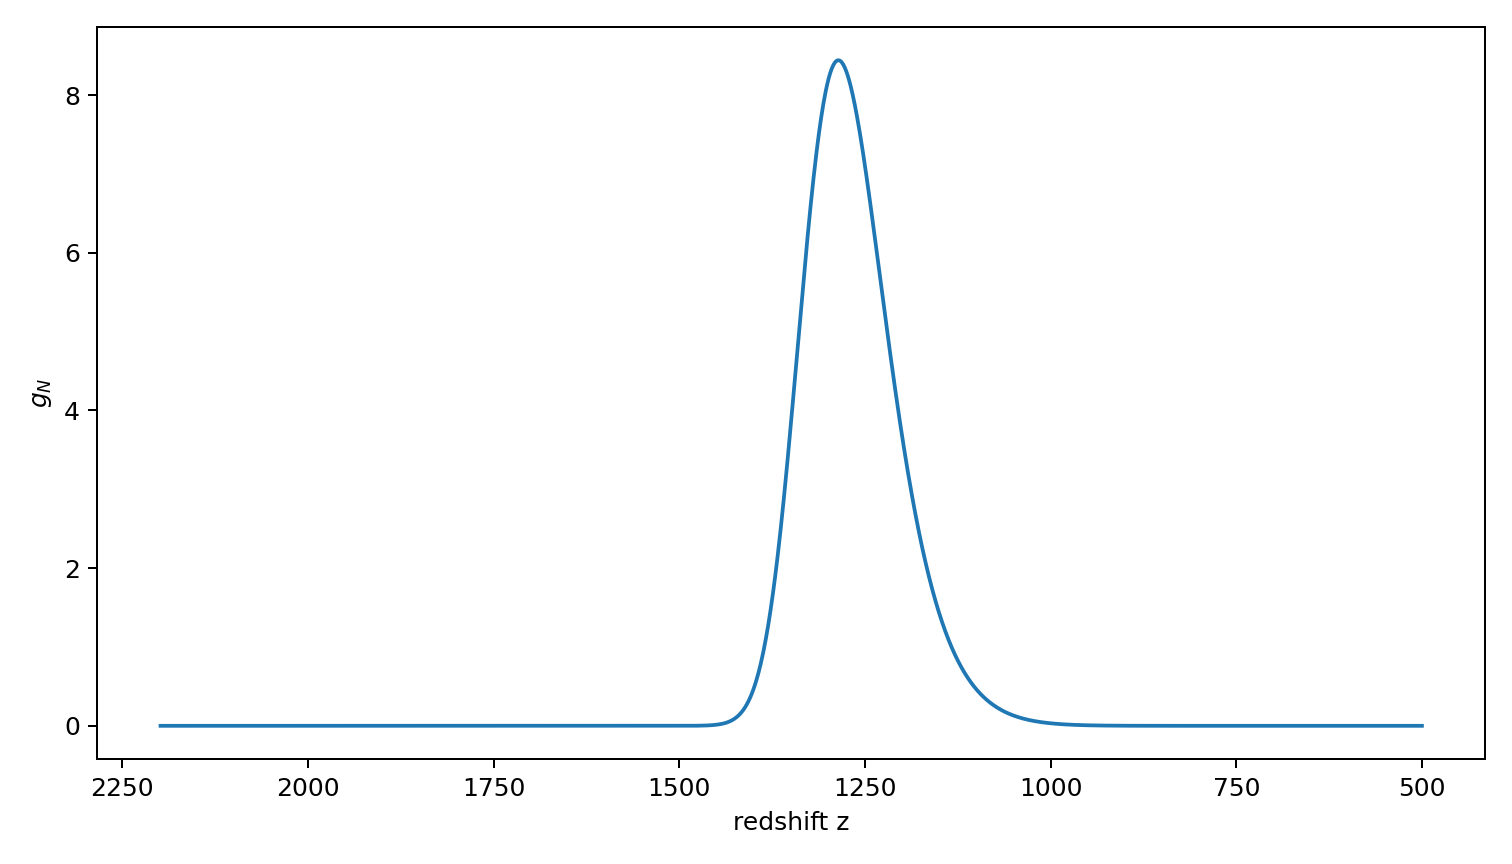
\includegraphics[width=0.88\linewidth]{figures/cmb/primary_cmb_visibility.png}
\caption{The controlled Saha visibility function in $d\log a$ measure.  The construction omits multilevel recombination, helium corrections beyond the fixed hydrogen fraction, and reionization.}
\label{fig:pcmb-visibility}
\end{figure}

\section{Metric conventions and Einstein closure}

Use conformal Newtonian gauge,
\begin{equation}
 ds^2=a^2(\eta)
 \left[-(1+2\Psi)d\eta^2+(1-2\Phi)d\mathbf x^2\right].
 \label{eq:pcmb-newtonian-gauge}
\end{equation}
Let
\begin{equation}
 \mathcal Q=\sum_s(\rho_s+p_s)\theta_s,
 \qquad
 \mathcal A=\sum_s(\rho_s+p_s)\sigma_s,
 \label{eq:pcmb-total-momentum-anis}
\end{equation}
where all densities are expressed in present critical-density units and $k$ is measured in $H_0$.  The implemented momentum and shear equations are
\begin{equation}
 \Phi'+\mathcal H\Psi
 =\frac{3}{2}\frac{a^2}{k^2}\mathcal Q,
 \label{eq:pcmb-einstein-momentum}
\end{equation}
\begin{equation}
 \Phi-\Psi
 =\frac{9}{2}\frac{a^2}{k^2}\mathcal A.
 \label{eq:pcmb-einstein-shear}
\end{equation}
The energy equation is not imposed after every step.  It is retained as an independent residual,
\begin{equation}
 \mathcal C_E
 :=k^2\Phi
 +3\mathcal H(\Phi'+\mathcal H\Psi)
 +\frac{3}{2}a^2\delta\rho.
 \label{eq:pcmb-energy-constraint}
\end{equation}
The largest relative accepted-state residual in the main run is
\begin{equation}
 \boxed{
 \epsilon_E=7.5049074572\times10^{-4}.}
 \label{eq:pcmb-energy-residual}
\end{equation}
The dedicated refinement runs reduce the largest accepted-state residual to $1.2091040\times10^{-4}$ on their common sample.

\section{Adiabatic production-surface data}

The perturbations are matched at $a=a_\star$ using one adiabatic mode.  Let
\begin{equation}
 \frac{\delta_s}{1+w_s}=C_\star
 \label{eq:pcmb-adiabatic-condition}
\end{equation}
for every populated species, and choose $\Phi'_\star=0$.  With $\Phi_\star=\Psi_\star=1$ as an intermediate normalization, the common velocity is
\begin{equation}
 \theta_\star
 =\frac{k^2\mathcal H_\star\Psi_\star}
 {\frac32a_\star^2\sum_s(\rho_s+p_s)},
 \label{eq:pcmb-initial-velocity}
\end{equation}
while the energy equation fixes
\begin{equation}
 C_\star
 =-
 \frac{k^2\Phi_\star+3\mathcal H_\star^2\Psi_\star}
 {\frac32a_\star^2\sum_s(\rho_s+p_s)}.
 \label{eq:pcmb-initial-density}
\end{equation}
Thus
\begin{equation}
 \delta_b=C_\star,
 \qquad
 \delta_\gamma=\delta_\nu=\frac43C_\star,
 \qquad
 \delta_D=(1+w_D)C_\star.
 \label{eq:pcmb-species-initial-density}
\end{equation}
The source functions are finally divided by the comoving-curvature normalization
\begin{equation}
 \mathcal R_\star=\Phi_\star-\frac13C_\star.
 \label{eq:pcmb-curvature-normalization}
\end{equation}

This is a declared matching condition on the production hypersurface.  The microscopic inhomogeneous crossing has not yet been solved, so the calculation does not claim that the full theory uniquely selects this adiabatic state.

\section{Tight-coupling stage}

From $a_\star$ to
\begin{equation}
 a_{\rm sw}=6.8\times10^{-4},
 \label{eq:pcmb-tight-switch}
\end{equation}
photons and baryons are evolved as one tight-coupled velocity $\theta$.  Set
\begin{equation}
 R_b(a)=\frac{3\rho_b}{4\rho_\gamma}
 =\frac{3\Omega_{b0}a}{4\Omega_{\gamma0}}.
 \label{eq:pcmb-baryon-loading}
\end{equation}
The leading brightness moments are
\begin{equation}
 F_{\gamma1}=\frac{4\theta}{3k},
 \qquad
 F_{\gamma2}=\frac{32\theta}{45\dot\kappa}.
 \label{eq:pcmb-tight-brightness}
\end{equation}
The common Euler equation is
\begin{equation}
 \theta'
 =-\mathcal H\frac{R_b}{1+R_b}\theta
 +k^2\left[
 \frac{\delta_\gamma}{4(1+R_b)}
 +\Psi
 +\frac{R_b}{1+R_b}c_b^2\delta_b
 \right].
 \label{eq:pcmb-tight-euler}
\end{equation}
The continuity equations are
\begin{equation}
 \delta_b'=-\theta+3\Phi',
 \qquad
 \delta_\gamma'=-\frac43\theta+4\Phi'.
 \label{eq:pcmb-tight-continuity}
\end{equation}
At $a_{\rm sw}$, the photon quadrupole is matched into the full hierarchy, and the scalar polarization moments are initialized by
\begin{equation}
 G_{\gamma0}=\frac54F_{\gamma2},
 \qquad
 G_{\gamma2}=\frac14F_{\gamma2}.
 \label{eq:pcmb-polarization-matching}
\end{equation}
This matching prescription is part of the controlled approximation and is tested through the multipole-refinement audit below.

\section{Photon temperature and polarization hierarchy}

Expand the photon temperature brightness and scalar polarization brightness as
\begin{equation}
 F_\gamma(\mu)=\sum_{\ell\geq0}(-i)^\ell(2\ell+1)F_{\gamma\ell}P_\ell(\mu),
 \label{eq:pcmb-photon-expansion}
\end{equation}
\begin{equation}
 G_\gamma(\mu)=\sum_{\ell\geq0}(-i)^\ell(2\ell+1)G_{\gamma\ell}P_\ell(\mu).
 \label{eq:pcmb-polarization-expansion}
\end{equation}
The conventions are
\begin{equation}
 F_{\gamma0}=\delta_\gamma,
 \qquad
 F_{\gamma1}=\frac{4\theta_\gamma}{3k},
 \qquad
 F_{\gamma2}=2\sigma_\gamma.
 \label{eq:pcmb-photon-moment-convention}
\end{equation}
Define the Thomson quadrupole source
\begin{equation}
 \Pi_\gamma=F_{\gamma2}+G_{\gamma0}+G_{\gamma2}.
 \label{eq:pcmb-pi-source}
\end{equation}
The implemented temperature equations are
\begin{equation}
 F_{\gamma0}'=-kF_{\gamma1}+4\Phi',
 \label{eq:pcmb-gamma-zero}
\end{equation}
\begin{equation}
 F_{\gamma1}'
 =\frac{k}{3}(F_{\gamma0}-2F_{\gamma2})
 +\frac{4k}{3}\Psi
 +\dot\kappa\left(\frac{4\theta_b}{3k}-F_{\gamma1}\right),
 \label{eq:pcmb-gamma-one}
\end{equation}
\begin{equation}
 F_{\gamma2}'
 =\frac{2k}{5}\left(F_{\gamma1}-\frac34F_{\gamma3}\right)
 -\dot\kappa\left(F_{\gamma2}-\frac1{10}\Pi_\gamma\right),
 \label{eq:pcmb-gamma-two}
\end{equation}
\begin{equation}
 F_{\gamma\ell}'
 =\frac{k}{2\ell+1}
 \left[\ell F_{\gamma,\ell-1}-(\ell+1)F_{\gamma,\ell+1}\right]
 -\dot\kappa F_{\gamma\ell},
 \qquad \ell\geq3.
 \label{eq:pcmb-gamma-general}
\end{equation}
The polarization equations are
\begin{equation}
 G_{\gamma0}'
 =-kG_{\gamma1}
 -\dot\kappa\left(G_{\gamma0}-\frac12\Pi_\gamma\right),
 \label{eq:pcmb-pol-zero}
\end{equation}
\begin{equation}
 G_{\gamma1}'
 =\frac{k}{3}(G_{\gamma0}-2G_{\gamma2})-\dot\kappa G_{\gamma1},
 \label{eq:pcmb-pol-one}
\end{equation}
\begin{equation}
 G_{\gamma2}'
 =\frac{2k}{5}\left(G_{\gamma1}-\frac34G_{\gamma3}\right)
 -\dot\kappa\left(G_{\gamma2}-\frac1{10}\Pi_\gamma\right),
 \label{eq:pcmb-pol-two}
\end{equation}
with the collisionally damped free-streaming recurrence for $\ell\geq3$.

The main solve uses
\begin{equation}
 L_\gamma=L_E=7.
 \label{eq:pcmb-photon-lmax}
\end{equation}
At the angular boundary, a spherical-Bessel recurrence estimates the next multipole using the free-streaming phase accumulated from the tight-coupling switch.

\section{Baryons and massless neutrinos}

After the switch, baryons obey
\begin{equation}
 \delta_b'=-\theta_b+3\Phi',
 \label{eq:pcmb-baryon-continuity}
\end{equation}
\begin{equation}
 \theta_b'
 =-\mathcal H\theta_b
 +c_b^2k^2\delta_b
 +\frac{4\rho_\gamma}{3\rho_b}\dot\kappa(\theta_\gamma-\theta_b)
 +k^2\Psi.
 \label{eq:pcmb-baryon-euler}
\end{equation}
The controlled thermal model keeps baryons at the photon temperature through recombination and cools them adiabatically afterward.  The baryon pressure term is numerically negligible for the primary acoustic dynamics but is retained.

Massless neutrinos use the collisionless brightness hierarchy
\begin{equation}
 F_{\nu0}'=-kF_{\nu1}+4\Phi',
 \label{eq:pcmb-nu-zero}
\end{equation}
\begin{equation}
 F_{\nu1}'=\frac{k}{3}(F_{\nu0}-2F_{\nu2})+\frac{4k}{3}\Psi,
 \label{eq:pcmb-nu-one}
\end{equation}
\begin{equation}
 F_{\nu\ell}'
 =\frac{k}{2\ell+1}
 \left[\ell F_{\nu,\ell-1}-(\ell+1)F_{\nu,\ell+1}\right],
 \qquad \ell\geq2,
 \label{eq:pcmb-nu-general}
\end{equation}
with
\begin{equation}
 L_\nu=6.
 \label{eq:pcmb-nu-lmax}
\end{equation}
The terminal recurrence uses the total free-streaming phase accumulated from $a_\star$, not merely the post-switch phase.  This distinction is required for stable early-time neutrino closure.

\section{Massive refinement hierarchy}

For every retained $(h,q)$ node, write
\begin{equation}
 \mathcal F_h(k,q,\mu,\eta)
 =\sum_{\ell\geq0}(-i)^\ell(2\ell+1)F_{h\ell}P_\ell(\mu),
 \label{eq:pcmb-dark-multipole-expansion}
\end{equation}
with
\begin{equation}
 D_h(q)=\frac{d\log\bar f_h}{d\log q},
 \qquad
 v_h(q,a)=\frac{q}{\epsilon_h(q,a)}.
 \label{eq:pcmb-dark-velocity-slope}
\end{equation}
The hierarchy is
\begin{equation}
 F_{h0}'=-kv_hF_{h1}-\Phi'D_h,
 \label{eq:pcmb-dark-zero}
\end{equation}
\begin{equation}
 F_{h1}'
 =\frac{kv_h}{3}(F_{h0}-2F_{h2})
 -\frac{k}{3v_h}\Psi D_h,
 \label{eq:pcmb-dark-one}
\end{equation}
\begin{equation}
 F_{h\ell}'
 =\frac{kv_h}{2\ell+1}
 \left[\ell F_{h,\ell-1}-(\ell+1)F_{h,\ell+1}\right],
 \qquad \ell\geq2.
 \label{eq:pcmb-dark-general}
\end{equation}
The sign in \eqref{eq:pcmb-dark-zero} is fixed so that the massless limit $D_h=-4$ reproduces the photon gravitational source $+4\Phi'$.

The massive density, pressure, momentum, and shear moments are reconstructed from the same hierarchy.  For example,
\begin{equation}
 \delta\rho_D
 =\frac{1}{2\pi^2a^4}
 \sum_hd_h\int q^2\epsilon_h\bar f_hF_{h0}\,dq,
 \label{eq:pcmb-dark-delta-rho}
\end{equation}
\begin{equation}
 \mathcal Q_D
 =\frac{k}{2\pi^2a^4}
 \sum_hd_h\int q^3\bar f_hF_{h1}\,dq,
 \label{eq:pcmb-dark-momentum}
\end{equation}
\begin{equation}
 \mathcal A_D
 =\frac{1}{3\pi^2a^4}
 \sum_hd_h\int\frac{q^4}{\epsilon_h}\bar f_hF_{h2}\,dq.
 \label{eq:pcmb-dark-shear}
\end{equation}
The main CMB solve uses $L_D=2$.  The refinement audit increases the photon, polarization, neutrino, and dark angular cutoffs simultaneously and finds a source discrepancy below one percent.

\section{Numerical phase space and integration}

The main deterministic state contains
\begin{center}
\begin{tabular}{lr}
\toprule
component & resolution\\
\midrule
wavenumbers & 101\\
retained refinement levels & 7\\
momentum nodes per level & 2\\
total massive phase-space nodes & 14\\
photon temperature multipoles & $0\leq\ell\leq7$\\
photon polarization multipoles & $0\leq\ell\leq7$\\
massless-neutrino multipoles & $0\leq\ell\leq6$\\
massive refinement multipoles & $0\leq\ell\leq2$\\
\bottomrule
\end{tabular}
\end{center}
The equations are integrated in $N=\log a$ by fourth-order Runge--Kutta.  The tight-coupling stage uses $\Delta N\simeq3.5\times10^{-3}$ and the full collision stage uses $\Delta N\simeq8.0\times10^{-4}$.  Source records extend to
\begin{equation}
 a_{\rm end}=1.55\times10^{-3},
 \label{eq:pcmb-end-scale}
\end{equation}
which lies beyond the visibility peak.

The solved source functions contain visible acoustic oscillations over the complete $k$ interval.
\begin{figure}[htbp]
\centering
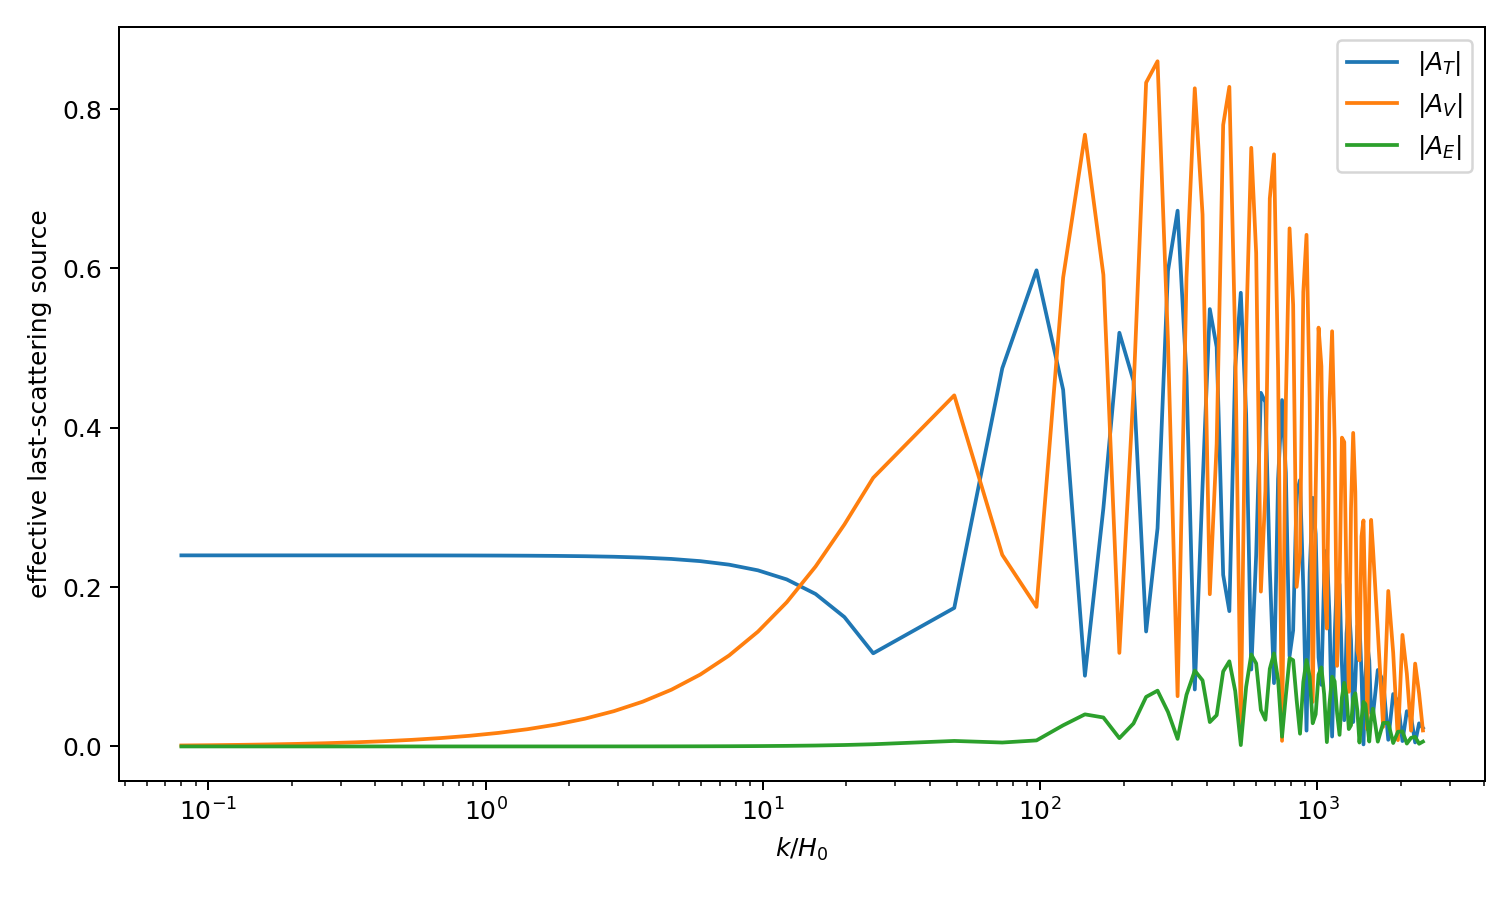
\includegraphics[width=0.88\linewidth]{figures/cmb/primary_cmb_sources.png}
\caption{Effective last-scattering temperature, velocity, and polarization source amplitudes.  The high-$k$ oscillations are sampled on the 101-mode Einstein--Boltzmann grid and spline-interpolated only at the final projection stage.}
\label{fig:pcmb-sources}
\end{figure}

\section{Finite-width last-scattering projection}

Define
\begin{equation}
 \Theta_0=\frac14F_{\gamma0}.
 \label{eq:pcmb-temperature-monopole}
\end{equation}
The source amplitudes in $dN$ measure are
\begin{equation}
 S_T
 =g_N\left(\Theta_0+\Psi+\frac1{16}\Pi_\gamma\right)
 +e^{-\tau}(\Psi_N-\Phi_N),
 \label{eq:pcmb-temperature-source}
\end{equation}
\begin{equation}
 S_V=g_N\frac{\theta_b}{k},
 \label{eq:pcmb-velocity-source}
\end{equation}
\begin{equation}
 S_E=\frac{3}{16}g_N\Pi_\gamma.
 \label{eq:pcmb-polarization-source}
\end{equation}
Their normalized integrated amplitudes are
\begin{equation}
 A_X(k)=\frac{1}{\mathcal R_\star}\int S_X(k,N)\,dN,
 \qquad
 X\in\{T,V,E\}.
 \label{eq:pcmb-integrated-sources}
\end{equation}

Let the visibility-weighted distance and width be
\begin{equation}
 \chi_\star
 =\frac{\int g_N\chi\,dN}{\int g_N\,dN},
 \qquad
 \sigma_\chi^2
 =\frac{\int g_N(\chi-\chi_\star)^2dN}{\int g_NdN}.
 \label{eq:pcmb-source-distance-width}
\end{equation}
The numerical values are
\begin{equation}
 \boxed{
 H_0\chi_\star=3.1438585561,
 \qquad
 H_0\sigma_\chi=2.3136123623\times10^{-3}.}
 \label{eq:pcmb-distance-width-values}
\end{equation}
The finite-width projection used here is
\begin{equation}
 \Delta_\ell^T(k)
 =e^{-k^2\sigma_\chi^2/2}
 \left[A_T(k)j_\ell(k\chi_\star)
 +A_V(k)j_\ell'(k\chi_\star)\right],
 \label{eq:pcmb-temperature-transfer}
\end{equation}
\begin{equation}
 \Delta_\ell^E(k)
 =e^{-k^2\sigma_\chi^2/2}
 \sqrt{\frac{(\ell+2)!}{(\ell-2)!}}
 A_E(k)\frac{j_\ell(k\chi_\star)}{(k\chi_\star)^2}.
 \label{eq:pcmb-e-transfer}
\end{equation}
This is a controlled narrow-source approximation.  A precision implementation would retain the complete time dependence inside the line-of-sight integral rather than compressing the source to $(A_T,A_V,A_E,\chi_\star,\sigma_\chi)$.

For
\begin{equation}
 \mathcal P_{\mathcal R}(k)
 =A_s\left(\frac{k}{k_\star}\right)^{n_s-1},
 \label{eq:pcmb-primordial-spectrum}
\end{equation}
with $A_s=2.1\times10^{-9}$, $n_s=0.965$, and $k_\star=0.05\,\mathrm{Mpc}^{-1}$, the angular spectra are
\begin{equation}
 C_\ell^{XY}
 =4\pi\int d\log k\,
 \mathcal P_{\mathcal R}(k)
 \Delta_\ell^X(k)\Delta_\ell^Y(k),
 \qquad
 X,Y\in\{T,E\}.
 \label{eq:pcmb-angular-spectra}
\end{equation}

\section{Acoustic and polarization results}

The visibility-peak sound horizon is
\begin{equation}
 H_0r_s=0.02913803155,
 \label{eq:pcmb-sound-horizon}
\end{equation}
and the geometric acoustic ruler is
\begin{equation}
 \boxed{
 \ell_A=\pi\frac{\chi_{\rm vis}}{r_s}=339.055741.}
 \label{eq:pcmb-acoustic-ruler}
\end{equation}
The first three resolved TT acoustic maxima above $\ell=80$ occur at
\begin{equation}
 \boxed{
 \ell_1=252,
 \qquad
 \ell_2=608,
 \qquad
 \ell_3=904.}
 \label{eq:pcmb-peak-positions}
\end{equation}
Their spacing is consistent with the geometric ruler to a relative discrepancy of $4.9975\times10^{-2}$ in the declared projection.

The first peak has
\begin{equation}
 \boxed{
 D_{\ell_1}^{TT}
 :=\frac{\ell_1(\ell_1+1)}{2\pi}C_{\ell_1}^{TT}T_{\gamma0}^2
 =6163.119890\,\mu\mathrm K^2.}
 \label{eq:pcmb-first-peak-amplitude}
\end{equation}
Selected template values are
\begin{center}
\begin{tabular}{rrrr}
\toprule
$\ell$ & $D_\ell^{TT}$ [$\mu$K$^2$] & $D_\ell^{EE}$ [$\mu$K$^2$] & $D_\ell^{TE}$ [$\mu$K$^2$]\\
\midrule
100 & 1220.174 & 0.289 & -1.418\\
200 & 4733.471 & 0.428 & -16.260\\
252 & 6163.120 & 0.459 & 17.919\\
500 & 2395.207 & 8.980 & -45.853\\
608 & 3467.906 & 4.787 & 27.666\\
904 & 3099.722 & 9.410 & -46.574\\
1000 & 1904.695 & 11.920 & 58.657\\
1500 & 343.904 & 15.671 & -25.350\\
2000 & 138.183 & 1.915 & 2.085\\
2500 & 10.197 & 1.762 & -0.480\\
\bottomrule
\end{tabular}
\end{center}
The temperature--polarization cross spectrum satisfies the Cauchy bound over every stored multipole,
\begin{equation}
 \max_\ell\frac{|C_\ell^{TE}|}{\sqrt{C_\ell^{TT}C_\ell^{EE}}}
 =0.9948225265<1.
 \label{eq:pcmb-te-cauchy}
\end{equation}

\begin{figure}[htbp]
\centering
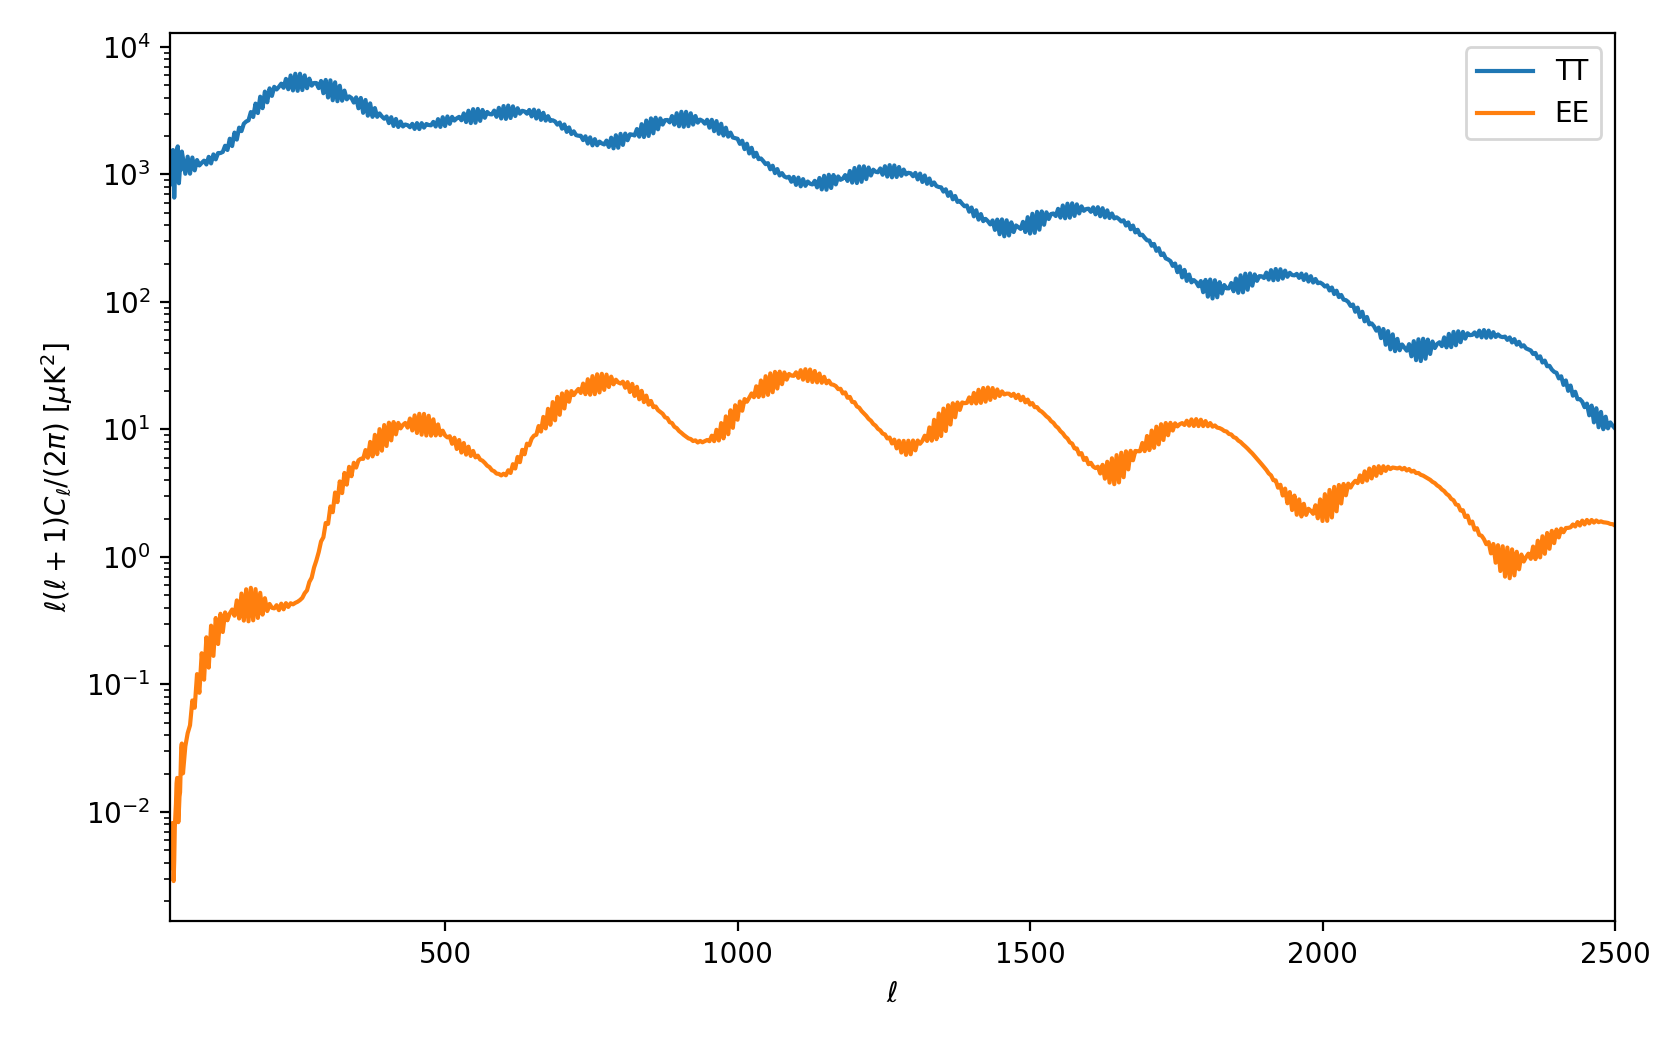
\includegraphics[width=0.90\linewidth]{figures/cmb/primary_cmb_tt_ee_acoustic.png}
\caption{Controlled recombination-era TT and EE templates.  The plotted range begins at $\ell=30$ because reionization and late integrated sources are not included.}
\label{fig:pcmb-tt-ee}
\end{figure}

\begin{figure}[htbp]
\centering
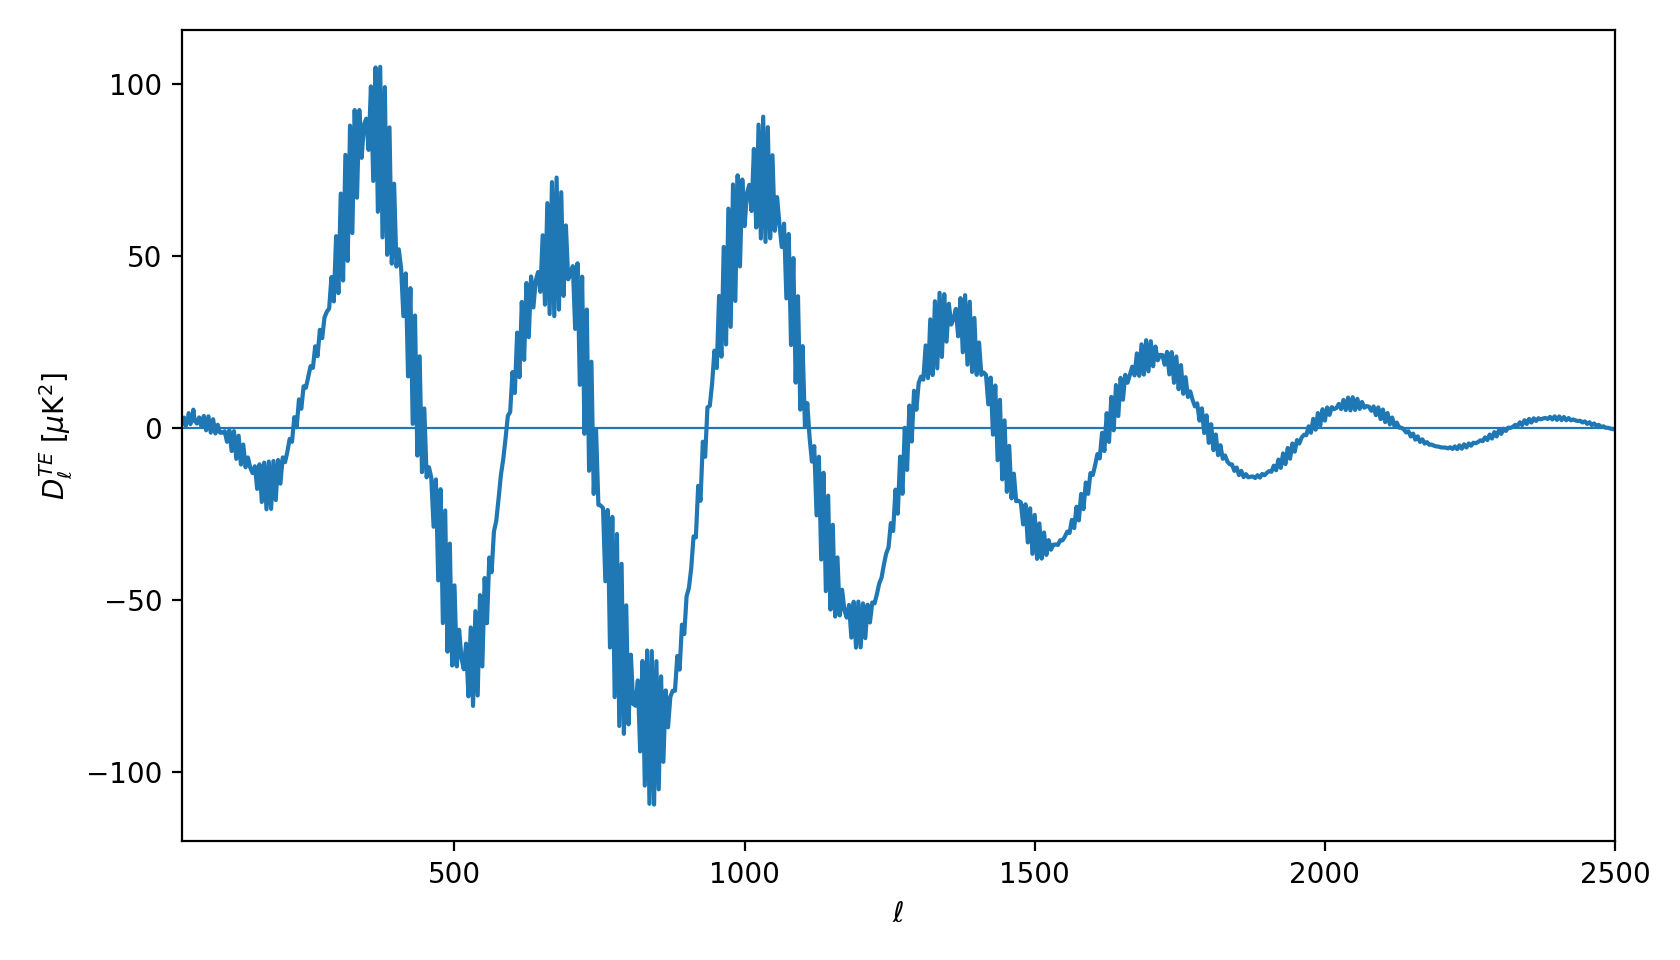
\includegraphics[width=0.90\linewidth]{figures/cmb/primary_cmb_te_acoustic.png}
\caption{The controlled TE template alternates sign across the acoustic series, reflecting the relative phase of photon compression, velocity, and polarization.}
\label{fig:pcmb-te}
\end{figure}

The finite source width suppresses high multipoles.  At $\ell=3000$, the declared Gaussian thickness factor is
\begin{equation}
 \exp\left[-\frac12
 \left(\frac{\ell\sigma_\chi}{\chi_\star}\right)^2\right]_{\ell=3000}
 =0.08741675187.
 \label{eq:pcmb-thickness-factor}
\end{equation}

\section{Convergence and verification}

The main deterministic audit contains
\begin{equation}
 \boxed{
 20\ \mathrm{PASS},
 \qquad
 0\ \mathrm{FAIL}.}
 \label{eq:pcmb-main-checks}
\end{equation}
A separate convergence audit adds
\begin{equation}
 \boxed{
 4\ \mathrm{PASS},
 \qquad
 0\ \mathrm{FAIL}.}
 \label{eq:pcmb-convergence-checks}
\end{equation}
The combined calculation therefore records
\begin{equation}
 \boxed{
 24\ \mathrm{PASS},
 \qquad
 0\ \mathrm{FAIL}.}
 \label{eq:pcmb-total-checks}
\end{equation}
The principal refinement differences are
\begin{center}
\begin{tabular}{lr}
\toprule
control & relative discrepancy\\
\midrule
momentum quadrature & $1.81645\times10^{-4}$\\
photon--neutrino--dark multipole truncation & $6.48202\times10^{-3}$\\
time step & $2.19752\times10^{-6}$\\
accepted-state Einstein constraint & $1.20910\times10^{-4}$\\
\bottomrule
\end{tabular}
\end{center}
The free-streaming spherical-Bessel identity is reproduced with maximum residual
\begin{equation}
 \epsilon_{\rm fs}=1.35046\times10^{-6}
 \label{eq:pcmb-free-streaming-residual}
\end{equation}
in the finite-difference derivative audit.  Median held-out source-interpolation errors are
\begin{equation}
 \epsilon_{A_T}=1.38235\times10^{-2},
 \qquad
 \epsilon_{A_V}=1.45514\times10^{-2},
 \qquad
 \epsilon_{A_E}=1.42026\times10^{-2}.
 \label{eq:pcmb-source-interpolation-errors}
\end{equation}
These source errors, together with the narrow-source projection, dominate over the time-step and momentum-quadrature errors in the current spectra.

\section{Closure ledger}

\begin{center}
\begin{tabular}{>{\raggedright\arraybackslash}p{0.47\linewidth}>{\raggedright\arraybackslash}p{0.21\linewidth}>{\raggedright\arraybackslash}p{0.24\linewidth}}
\toprule
statement & status & boundary\\
\midrule
photon temperature hierarchy with Thomson scattering & closed controlled & scalar linear perturbations\\
scalar polarization hierarchy and nonzero $E$ source & closed controlled & no $B$ modes\\
baryon drag and acoustic loading & closed controlled & simple baryon thermal history\\
massless-neutrino hierarchy and anisotropic stress & closed controlled & fixed $\Omega_{\nu0}$\\
massive refinement hierarchy through recombination & closed controlled & seven levels, fourteen phase nodes\\
Einstein momentum and shear coupling & closed controlled & Newtonian gauge\\
energy-constraint audit & numerically controlled & not projected after each step\\
Saha visibility and finite source width & closed conditional & no multilevel recombination\\
recombination-era TT, TE, EE acoustic templates & numerically closed & narrow-source projection\\
low-$\ell$ TT, TE, EE prediction & open & reionization and late integrated sources\\
precision recombination and helium kinetics & open & external atomic network\\
full line-of-sight source integration & open & production-grade transfer solver\\
lensing remapping and nonlinear late-time sources & open & nonlinear structure\\
joint likelihood and parameter inference & open & observational data and nuisance model\\
microscopic perturbation matching at production & open & nonlinear inhomogeneous crossing\\
\bottomrule
\end{tabular}
\end{center}

\clearpage
\section{Synthesis and scope}

The scale-covariant distribution now enters one coupled chain,
\begin{equation}
 \boxed{
 \begin{gathered}
 \bar f_h(q)
 \longrightarrow
 \{F_{h\ell},F_{\nu\ell},F_{\gamma\ell},G_{\gamma\ell},\delta_b,\theta_b\}
 \\
 \longrightarrow
 \{\Phi,\Psi,g_N\}
 \longrightarrow
 \{A_T,A_V,A_E\}
 \longrightarrow
 \{C_\ell^{TT},C_\ell^{TE},C_\ell^{EE}\}.
 \end{gathered}}
 \label{eq:pcmb-result-chain}
\end{equation}
No dark-sector parameter is changed between production, background expansion, late-time collisionless structure, and the controlled primary-CMB calculation.

This closes the principal species-coupling gap at the level of a deterministic linear template.  A precision line-of-sight and thermal-history treatment still requires:
\begin{equation}
 \boxed{
 \begin{gathered}
 \text{replace Saha recombination by multilevel H/He kinetics},\\
 \text{derive the production-surface perturbation transfer},\\
 \text{add reionization, late ISW, and lensing remapping},\\
 \text{compute primary and late-time observables in one solver},\\
 \text{then perform a first joint likelihood without dark-sector retuning}.
 \end{gathered}}
 \label{eq:pcmb-open-requirements}
\end{equation}
